\documentclass[12pt]{article}%
\usepackage{amsfonts}
\usepackage{fancyhdr}
\usepackage{comment}
\usepackage[a4paper, top=2.5cm, bottom=2.5cm, left=2.2cm, right=2.2cm]%
{geometry}
\usepackage{times}
\usepackage{amsmath}
\usepackage{changepage}
\usepackage{amssymb}
\usepackage{graphicx}
\usepackage{url}%
\usepackage{xcolor}
\usepackage{amsmath} 
\setcounter{MaxMatrixCols}{30}
\newtheorem{theorem}{Theorem}
\newtheorem{acknowledgement}[theorem]{Acknowledgement}
\newtheorem{algorithm}[theorem]{Algorithm}
\newtheorem{axiom}{Axiom}
\newtheorem{case}[theorem]{Case}
\newtheorem{claim}[theorem]{Claim}
\newtheorem{conclusion}[theorem]{Conclusion}
\newtheorem{condition}[theorem]{Condition}
\newtheorem{conjecture}[theorem]{Conjecture}
\newtheorem{corollary}[theorem]{Corollary}
\newtheorem{criterion}[theorem]{Criterion}
\newtheorem{definition}[theorem]{Definition}
\newtheorem{example}[theorem]{Example}
\newtheorem{exercise}[theorem]{Exercise}
\newtheorem{lemma}[theorem]{Lemma}
\newtheorem{notation}[theorem]{Notation}
\newtheorem{problem}[theorem]{Problem}
\newtheorem{proposition}[theorem]{Proposition}
\newtheorem{remark}[theorem]{Remark}
\newtheorem{solution}[theorem]{Solution}
\newtheorem{summary}[theorem]{Summary}
\newenvironment{proof}[1][Proof]{\textbf{#1.} }{\ \rule{0.5em}{0.5em}}

\newcommand{\Q}{\mathbb{Q}}
\newcommand{\R}{\mathbb{R}}
\newcommand{\C}{\mathbb{C}}
\newcommand{\Z}{\mathbb{Z}}

\begin{document}

\title{CS280 Spring 2025 Assignment 1 \\ Part A}
\author{Basics}
\maketitle

\paragraph{Name: Chen Xuanxin}

\paragraph{Student ID: 2024233125}

\newpage

\subsubsection*{1. \textit{Maximum Likelihood Estimation} (10 points).}
Consider a dataset $\mathcal{D}$ consisting of $n$ independent and identically distributed samples:
\begin{equation}
    \mathcal{D} = \left\{ ((x^1_1, x^1_2), y^1), ((x^2_1, x^2_2), y^2), \ldots, ((x^n_1, x^n_2), y^n) \right\},
    \tag{1}
\end{equation}
where $(x^i_1, x^i_2) \in \mathbb{R}^2$ are input features and $y^i \in \mathbb{R}$ is an output. 
\\
Assume that every output $y^i$ in $\mathcal{D}$ is generated by inputting $(x^i_1, x^i_2)$ into a model:
\begin{equation}
    y = f_{\theta_1,\theta_2}(x_1, x_2) + \epsilon,
    \tag{2}
\end{equation}
where the function $f_{\theta_1,\theta_2}$ is a mapping from features $(x_1, x_2) \in \mathbb{R}^2$ to a value in $\mathbb{R}$, which has two parameters $\theta_1$ and $\theta_2$. Here we assume that the random noise $\epsilon \sim N(0,\sigma^2)$ is independent and distributed according to a Gaussian distribution with zero mean and variance $\sigma^2$.
\vspace{1em}
\\
(a) Show that the log likelihood of the data given the parameters is:
\begin{equation}
    l(\mathcal{D};\theta_1,\theta_2) = -\frac{1}{2\sigma^2}\sum_{i=1}^{n}(y^i-f_{\theta_1,\theta_2}(x^i_1,x^i_2))^2-n\log(\sqrt{2\pi}\sigma).
    \tag{3}
\end{equation}
Recall the probability density function of the Gaussian distribution $N(\mu,\sigma^2)$ is:
\begin{equation}
    p(x)=\frac{1}{\sqrt{2\pi}\sigma}\exp\left(-\frac{(x-\mu)^2}{2\sigma^2} \right).
    \tag{4}
\end{equation}
\vspace{1em}
\\
(b) To find the maximum likelihood estimates of $\theta_1$ and $\theta_2$ using gradient descent, compute the gradient of the log likelihood with respect to $\theta_1$ and $\theta_2$. Express you answer in terms of:
\begin{equation*}
    y^i, \enspace f_{\theta_1,\theta_2}(x^i_1, x^i_2), \enspace \frac{\partial}{\partial\theta_1}f_{\theta_1,\theta_2}(x^i_1, x^i_2), \enspace \frac{\partial}{\partial\theta_2}f_{\theta_1,\theta_2}(x^i_1, x^i_2)
\end{equation*}
\vspace{1em}
\\
(c) Given the learning rate $\eta$, what update rule would you use in gradient descent to \textit{maximize} the likelihood.

\pagebreak

\section{Answer for Maximum Likelihood Estimation}

\textbf{(a) Derivation of Log-Likelihood}  

Given the noise $\epsilon \sim N(0, \sigma^2)$, the conditional distribution of each sample $y^i$ is:
$$ y^i \mid x^i_1, x^i_2 \sim N\left(f_{\theta_1,\theta_2}(x^i_1, x^i_2), \sigma^2\right). $$

Using the probability density function of the Gaussian distribution (Equation (4)), the likelihood for a single sample is:
$$ p(y^i \mid x^i_1, x^i_2, \theta_1, \theta_2) = \frac{1}{\sqrt{2\pi}\sigma} \exp\left(-\frac{(y^i - f_{\theta_1,\theta_2}(x^i_1, x^i_2))^2}{2\sigma^2}\right). $$

Since the samples are independent and identically distributed (i.i.d.), the total likelihood is the product of individual likelihoods:
$$ L(\mathcal{D}; \theta_1, \theta_2) = \prod_{i=1}^n \frac{1}{\sqrt{2\pi}\sigma} \exp\left(-\frac{(y^i - f_{\theta_1,\theta_2}(x^i_1, x^i_2))^2}{2\sigma^2}\right). $$

Taking the logarithm and simplifying:
$$
\begin{aligned}
l(\mathcal{D}; \theta_1, \theta_2) &= \sum_{i=1}^n \ln\left( \frac{1}{\sqrt{2\pi}\sigma} \exp\left(-\frac{(y^i - f_{\theta_1,\theta_2}(x^i_1, x^i_2))^2}{2\sigma^2}\right) \right) \\
&= \sum_{i=1}^n \left( -\ln(\sqrt{2\pi}\sigma) - \frac{(y^i - f_{\theta_1,\theta_2}(x^i_1, x^i_2))^2}{2\sigma^2} \right) \\
&= -\frac{1}{2\sigma^2} \sum_{i=1}^n (y^i - f_{\theta_1,\theta_2}(x^i_1, x^i_2))^2 - n\ln(\sqrt{2\pi}\sigma).
\end{aligned}
$$

Thus, the log-likelihood is:
\begin{equation*}
    \textcolor{red}{l(\mathcal{D};\theta_1,\theta_2) = -\frac{1}{2\sigma^2}\sum_{i=1}^{n}(y^i-f_{\theta_1,\theta_2}(x^i_1,x^i_2))^2 -n\log(\sqrt{2\pi}\sigma)}
\end{equation*}    
% $$ \boxed{l(\mathcal{D};\theta_1,\theta_2) = -\frac{1}{2\sigma^2}\sum_{i=1}^{n}(y^i-f_{\theta_1,\theta_2}(x^i_1,x^i_2))^2 -n\log(\sqrt{2\pi}\sigma)}. $$


\textbf{(b) Gradient Computation}  

The partial derivative with respect to $\theta_1$ is:
$$
\begin{aligned}
\frac{\partial l}{\partial \theta_1} &= -\frac{1}{2\sigma^2} \sum_{i=1}^n \frac{\partial}{\partial \theta_1} \left( y^i - f_{\theta_1,\theta_2}(x^i_1, x^i_2) \right)^2 \\
&= -\frac{1}{2\sigma^2} \sum_{i=1}^n 2 \left( y^i - f_{\theta_1,\theta_2}(x^i_1, x^i_2) \right) \cdot \left(-\frac{\partial f_{\theta_1,\theta_2}}{\partial \theta_1}\right) \\
&= \frac{1}{\sigma^2} \sum_{i=1}^n \left( y^i - f_{\theta_1,\theta_2}(x^i_1, x^i_2) \right) \frac{\partial f_{\theta_1,\theta_2}}{\partial \theta_1}.
\end{aligned}
$$

Similarly, the partial derivative with respect to $\theta_2$ is:
$$ \frac{\partial l}{\partial \theta_2} = \frac{1}{\sigma^2} \sum_{i=1}^n \left( y^i - f_{\theta_1,\theta_2}(x^i_1, x^i_2) \right) \frac{\partial f_{\theta_1,\theta_2}}{\partial \theta_2}. $$

The gradient vector is:
\begin{equation*}
    \textcolor{red}{\nabla_{\theta_1, \theta_2} l = \left[ \frac{1}{\sigma^2} \sum_{i=1}^n \left( y^i - f_{\theta_1,\theta_2}(x^i_1, x^i_2) \right) \frac{\partial f_{\theta_1,\theta_2}}{\partial \theta_1}, \  \frac{1}{\sigma^2} \sum_{i=1}^n \left( y^i - f_{\theta_1,\theta_2}(x^i_1, x^i_2) \right) \frac{\partial f_{\theta_1,\theta_2}}{\partial \theta_2} \right]}
\end{equation*}

% $$ \boxed{\nabla_{\theta_1, \theta_2} l = \left[ \frac{1}{\sigma^2} \sum_{i=1}^n \left( y^i - f_{\theta_1,\theta_2}(x^i_1, x^i_2) \right) \frac{\partial f_{\theta_1,\theta_2}}{\partial \theta_1}, \  \frac{1}{\sigma^2} \sum_{i=1}^n \left( y^i - f_{\theta_1,\theta_2}(x^i_1, x^i_2) \right) \frac{\partial f_{\theta_1,\theta_2}}{\partial \theta_2} \right]}. $$


\textbf{(c) Gradient Descent Update Rule}  
To maximize the likelihood, we use gradient ascent. The update rule for parameters is:
$$ \theta_j^{(k+1)} = \theta_j^{(k)} + \eta \cdot \frac{\partial l}{\partial \theta_j}, \quad j=1,2. $$
Substituting the gradient expressions, we get:

\begin{equation*}
    \textcolor{red}{
        \theta_j^{(k+1)} = \theta_j^{(k)} + \frac{\eta}{\sigma^2} \sum_{i=1}^n \left( y^i - f_{\theta_1,\theta_2}(x^i_1, x^i_2) \right) \frac{\partial f_{\theta_1,\theta_2}}{\partial \theta_j}, \quad j=1,2
    }
\end{equation*}

\pagebreak

\subsubsection*{2. \textit{Loss Function} (10 points).}

Assume that a classifier is written as $H(x) = sign(F(x))$, where $H(x):\mathbb{R}^d \rightarrow \{-1, 1\}$, $sign()$ is a sign function, and $F(x): \mathbb{R}^d \rightarrow \mathbb{R}$. To obtain the parameters in $F(x)$, we need to minimize the loss function averaged over the training set: ${\textstyle \sum_{i}^{}}L(y^iF(x^i))$. Here $L$ is a function of $yF(x)$. For example, for linear classifiers, $F(x)=w_0 + {\textstyle \sum_{j=1}^{d}}w_jx_j$, and $yF(x) = y(w_0 + {\textstyle \sum_{j=1}^{d}}w_jx_j)$.
\vspace{1em}
\\
(a) Which loss functions below are appropriate to use in classification? For the ones that are not appropriate, explain why not. In general, what conditions does $L$ have to satisfy in order to be an appropriate loss function? The x axis is $yF(x)$, and the y axis is $L(yF(x))$.
\begin{figure}[htpb]
    \centering
    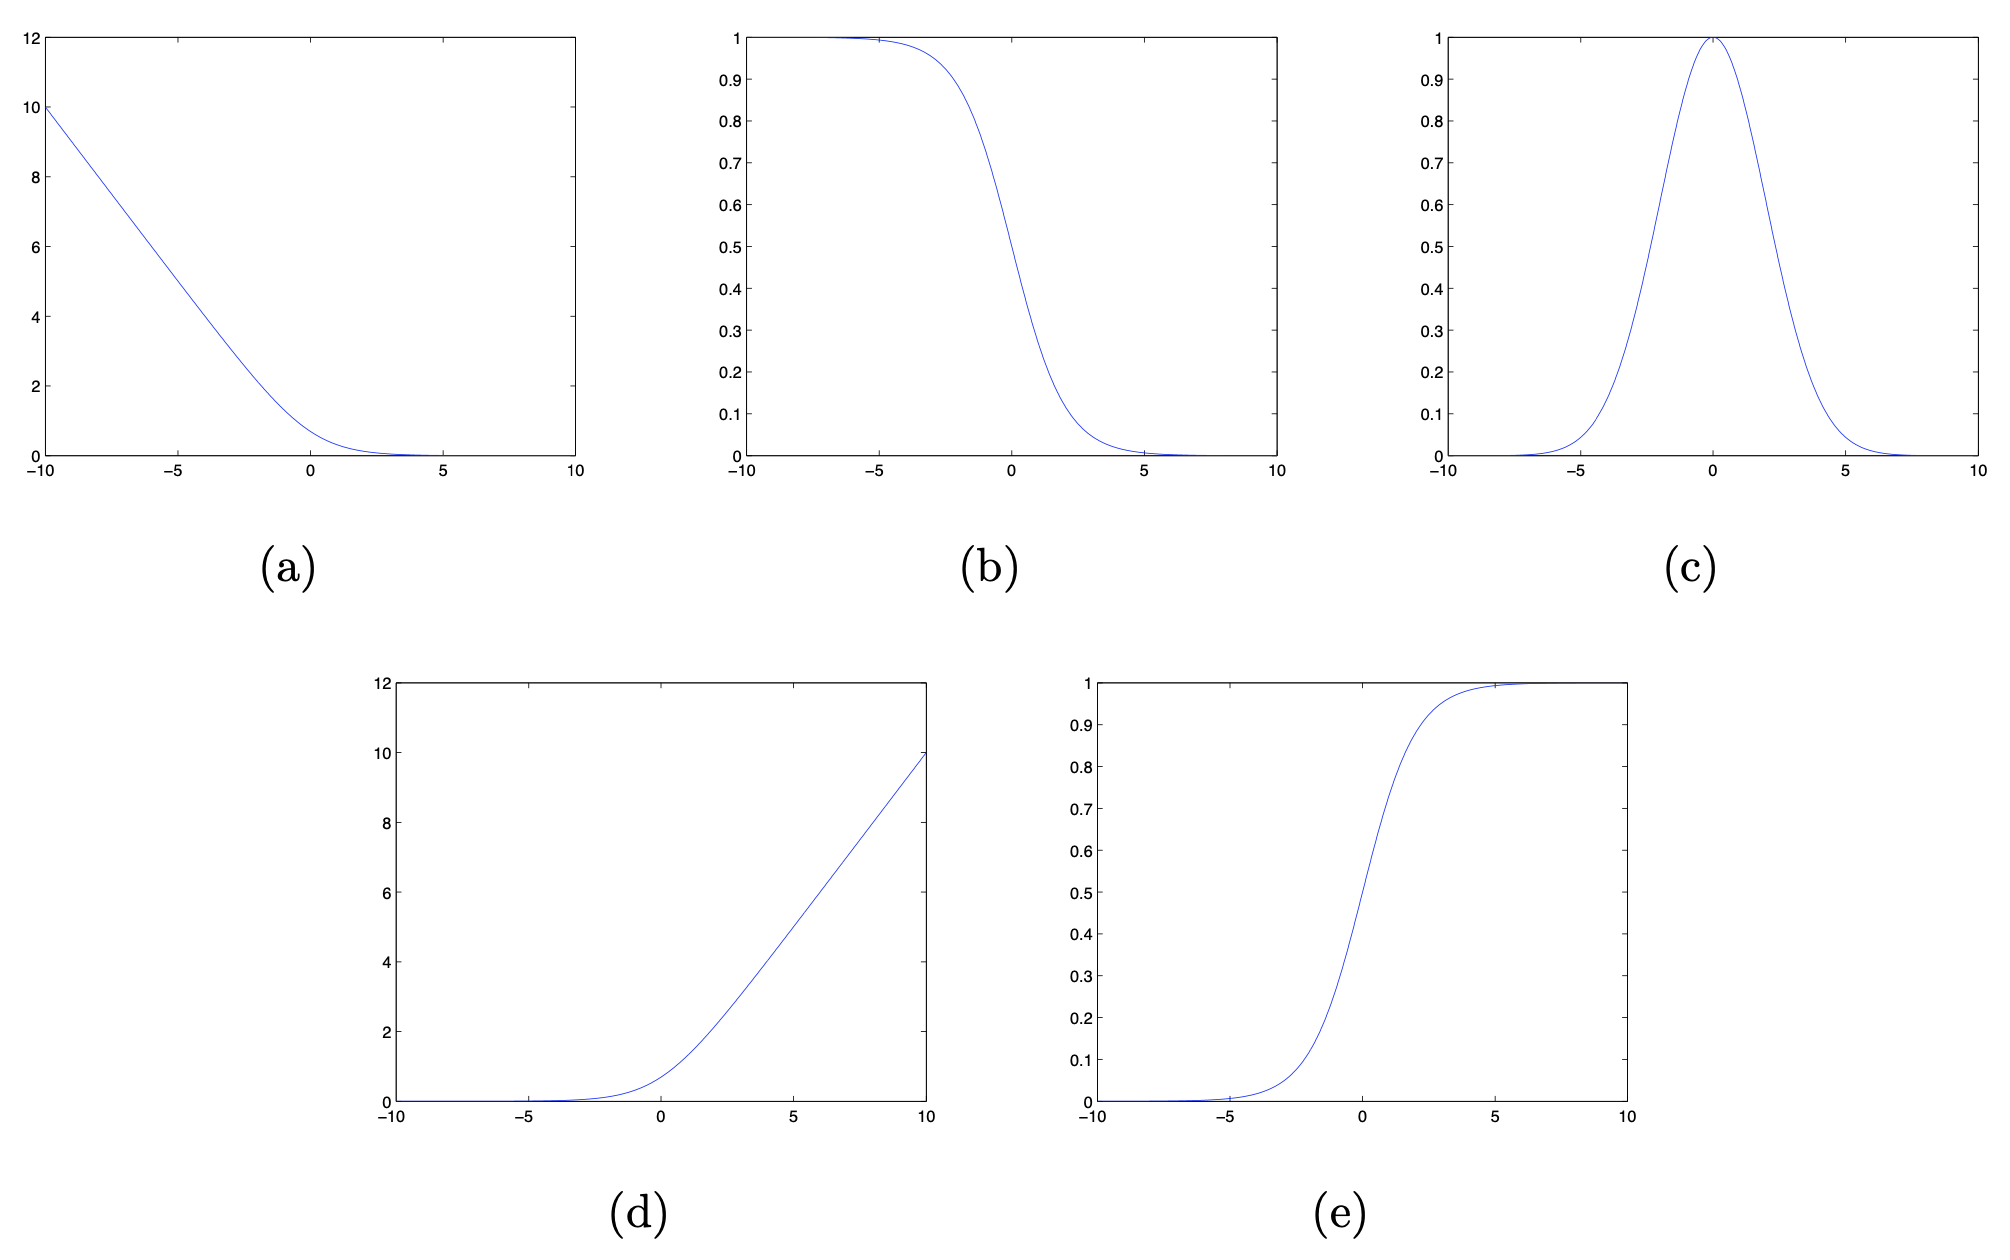
\includegraphics[scale=0.45]{partA_loss.png}
    \label{fig:enter-label}
\end{figure}
\vspace{1em}
\\
(b) Among the above loss functions appropriate to use in classification, which one is the most robust to outliers? Justify your answer.
\vspace{1em}
\\
(c) Let $F(x)=w_0+\sum_{j=1}^{d}w_jx_j$ and $L(yF(x))= \frac{1}{1+exp(yF(x))} $. Suppose you use gradient descent to obtain the optimal values for $w_0$ and $w_j$. Give the update rules for these parameters.
\pagebreak
\section{Answer for Loss Functions}
\subsubsection*{(a) Appropriate loss functions}

From the provided plots (a)--(e) (with the x-axis being $yF(x)$ and the y-axis being $L(yF(x))$), 
we see that only (a) and (b) are monotonically decreasing and approach 0 as $yF(x)\to +\infty$. 
These two satisfy the typical requirements for classification loss:
\begin{itemize}
  \item $L(t)\ge 0$ for all $t$,
  \item $L(t)$ is decreasing in $t$,
  \item $L(t)\to 0$ as $t\to +\infty$ (correct classification with large margin),
  \item $L(t)$ becomes large when $t\ll 0$ (incorrect classification with large negative margin).
\end{itemize}
\noindent
\textbf{Analysis of subfigures (a)-(e):}
\begin{table}[ht]
    \centering
    \begin{tabular}{|c|l|c|}
    \hline
    Subfigure & Characteristics & Appropriate? \\
    \hline
    (a) & Exponentially decreasing curve: $L \approx 10 \rightarrow 0$ as $yF(x)$ increases & \checkmark \\
    (b) & Saturated loss: Flat regions for $|yF(x)|>2$, sharp transition near $yF(x)=0$ & \checkmark \\
    (c) & Bell-shaped curve: Peaks at $yF(x)=0$ (\textit{opposite} to required monotonicity) & $\times$ \\
    (d) & Increasing linear function: $L \propto yF(x)$ (\textit{violates} the decreasing requirement) & $\times$ \\
    (e) & Logistic-like curve but reversed sign: does not decrease as $yF(x)$ grows & $\times$ \\
    \hline
    \end{tabular}
\end{table}

Only (a) and (b) are \emph{monotonically decreasing} in $yF(x)$ and approach 0 when $yF(x)\to +\infty$. 

Hence, (a) and (b) are appropriate for classification; (c), (d), and (e) are not.

\subsubsection*{(b) Robustness to outliers}

Among the appropriate loss functions, (a) resembles the exponential loss, while (b) resembles a logistic-type loss. 
The exponential loss $\exp(-yF(x))$ grows very large for highly negative margins and is therefore 
more sensitive to outliers. The logistic loss saturates more smoothly, making it more robust to outliers.
Hence, (b) is the most robust among them.

\subsubsection*{(c) Gradient descent updates for $L\bigl(yF(x)\bigr)=\frac{1}{1+\exp\bigl(yF(x)\bigr)}$}

Let the training set be $\{(x^i,\,y^i)\}_{i=1}^n$, where $y^i\in\{-1,+1\}$, and define 
\[
F(x^i) \;=\; w_0 \;+\;\sum_{j=1}^d w_j\,x_j^i.
\]
Then the loss for sample $i$ is
\[
L_i \;=\; L\bigl(y^i F(x^i)\bigr)
     \;=\; \frac{1}{1 + \exp\bigl(y^i F(x^i)\bigr)}.
\]
We want to minimize the sum $\displaystyle \sum_{i=1}^n L_i$.

\paragraph{Partial derivatives.}
Let $z_i = y^i F(x^i)$. Then
\[
L_i \;=\; \frac{1}{1 + e^{z_i}}, 
\quad
\frac{\partial L_i}{\partial z_i} 
=\; -\,\frac{e^{z_i}}{\bigl(1 + e^{z_i}\bigr)^2}
=\; -\,L_i\,(1 - L_i).
\]
Note also that 
\(\displaystyle \frac{\partial z_i}{\partial w_0} = y^i\),
and 
\(\displaystyle \frac{\partial z_i}{\partial w_j} = y^i\,x_j^i.\)

Hence,
\[
\frac{\partial L_i}{\partial w_0}
=\; \frac{\partial L_i}{\partial z_i}\,\frac{\partial z_i}{\partial w_0}
=\; -\,y^i\,L_i\,(1 - L_i),
\]
\[
\frac{\partial L_i}{\partial w_j}
=\; -\,y^i\,x_j^i\,L_i\,(1 - L_i).
\]

\paragraph{Gradient descent updates.}
Let $\alpha$ be the learning rate. Then the update rules for each iteration are:
\[
w_0 \;\leftarrow\; w_0 \;-\; \alpha \sum_{i=1}^n \frac{\partial L_i}{\partial w_0}
\;=\; w_0 \;+\; \alpha \sum_{i=1}^n 
     \Bigl[y^i\,L_i\,\bigl(1 - L_i\bigr)\Bigr],
\]
\[
w_j \;\leftarrow\; w_j \;-\; \alpha \sum_{i=1}^n \frac{\partial L_i}{\partial w_j}
\;=\; w_j \;+\; \alpha \sum_{i=1}^n 
     \Bigl[y^i\,x_j^i\,L_i\,\bigl(1 - L_i\bigr)\Bigr],
\]
where 
\(\displaystyle L_i = \frac{1}{1 + \exp\bigl(y^i F(x^i)\bigr)}.\)
\end{document}